% !TEX root = ../mechanics.tex
\section{关于气动中心的额外讨论}
在前面薄翼理论中,我们证明了气动中心不仅是
真实存在的,而且位置在翼型的四分之一的弦线
处。因此,我们可以增加一种新的方法来描述翼
型上的气动力和气动力矩,也就是气动力和气动
力矩通过气动中心。

对于大部分常规的翼型,不是很精确地说,气动
中心都是比较靠近四分之一弦线这个位置。只要
给出任意一个翼型的气动力系数曲线和气动力矩
系数曲线,我们都可以按照下面的方法计算出气
动中心的位置。考虑对四分之一弦线出取力矩和
升力的升力力矩系。将气动中心到前缘点的距离
记为
$c \overline{x}_{ac}$,
将气动中心记作ac,于是我们有
\[
	M'_{ac}=L'\left(c \overline{x}_{ac}-\frac{c}{4}\right)+M'_{\frac{c}{4}}
\]
上式两边同时除以
$q_\infty Sc$
我们得到
\[
	c_{m,ac}=c_l(\overline{x}_{ac}-\frac{1}{4})+c_{m,\frac{c}{4}}
\]
对上式两边同时对攻角$\alpha$取微分,我们有
\[
	\frac{\mathrm{d}c_{m,ax}}{\mathrm{d}\alpha}
	=\frac{\mathrm{d}c_l}{\mathrm{d}\alpha}(\overline{x}_{ac}-\frac{1}{4})
	+\frac{\mathrm{d}c_{m,\frac{c}{4}}}{\mathrm{d}\alpha}
\]
根据气动中心定义,有
\[
	\frac{\mathrm{d}c_{m,ac}}{\mathrm{d}\alpha}=0
\]
所以
\[
	0=\frac{\mathrm{d}c_l}{\mathrm{d}\alpha}(\overline{x}_{ac}-\frac{1}{4})
	+\frac{\mathrm{d}c_{m,\frac{c}{4}}}{\mathrm{d}\alpha}
\]
对于一个尚未达到失速的翼型,升力系数曲线和力矩系数曲线的
斜率都是一个常数,所以
\[
	\frac{\mathrm{d}c_l}{\mathrm{d}\alpha}=a_0 \qquad
	\frac{\mathrm{d}c_{m,\frac{c}{4}}}{\mathrm{d}\alpha}=m_0
\]
就得到了
\[
	0=a_0(\overline{x}_{ac}-\frac{1}{4})+m_0
\]
或者
\[
	\overline{x}_{ac}=-\frac{m_0}{a_0}+\frac{1}{4}
\]
这个方程证明了,对于一个有着线性的升力线和力矩线
的翼型来说,气动中心的位置就是固定的。当然,这还
给出了一个计算气动中心位置的方法。

\section{粘性流动:翼型阻力}
我们知道翼型的升力主要是翼面上的压强分布产生的;
翼面上的剪切力的分布在沿升力方向上的积分通常是
微不足道的。因此,升力可以通过无粘不可压流动结合
后缘点的库塔条件被精确地计算出来。当需要去预测
阻力的时候,这个方法得到的结果就是0 ,这个结果
和常见的场景是截然相反的,这就是达朗贝尔谬论。

直到粘性这个概念引入流动,这个悖论才被解决。
事实上,粘性完全是翼型产生阻力的原因。它通过
两种机制产生作用:
\begin{enumerate}
	\item 表面摩擦阻力,即主要由翼型表面上的剪切力分布产生的;
	\item 压差阻力,主要是由流动分离产生的,也叫做型阻;
\end{enumerate}
剪切力产生阻力是显而易见的,流动分离产生阻力是一个微妙
的现象,我们将在后面讨论。
\subsection{估计表面摩擦阻力:层流}
作为一种近似,我们假设一个翼型上的表面
摩擦阻力和一块平板上的表面摩擦阻力是一
样的,如图\ref{fig:plate}。
\begin{figure}[!ht]
	\centering
	% ! TEX root = ./Incompressible_Flow_Airfoil_2.tex

\tikzset{every picture/.style={line width=0.75pt}} %set default line width to 0.75pt        

\begin{tikzpicture}[x=0.75pt,y=0.75pt,yscale=-1,xscale=1]
%uncomment if require: \path (0,300); %set diagram left start at 0, and has height of 300

%Shape: Rectangle [id:dp8246665344533497] 
\draw  [fill={rgb, 255:red, 74; green, 144; blue, 226 }  ,fill opacity=1 ] (90.39,122.31) -- (540,122.31) -- (540,140) -- (90.39,140) -- cycle ;
%Curve Lines [id:da111522274445083] 
\draw  [dash pattern={on 4.5pt off 4.5pt}]  (90.39,122.31) .. controls (97.1,85.96) and (417.76,18.63) .. (530,20) ;
%Straight Lines [id:da9873373468406699] 
\draw [line width=3]    (280,130) -- (384,130) ;
\draw [shift={(390,130)}, rotate = 180] [fill={rgb, 255:red, 0; green, 0; blue, 0 }  ][line width=0.08]  [draw opacity=0] (16.97,-8.15) -- (0,0) -- (16.97,8.15) -- cycle    ;
%Straight Lines [id:da3618853648976492] 
\draw    (10,130) -- (78,130) ;
\draw [shift={(80,130)}, rotate = 180] [color={rgb, 255:red, 0; green, 0; blue, 0 }  ][line width=0.75]    (10.93,-3.29) .. controls (6.95,-1.4) and (3.31,-0.3) .. (0,0) .. controls (3.31,0.3) and (6.95,1.4) .. (10.93,3.29)   ;
%Straight Lines [id:da2969004979431211] 
\draw    (90,150) -- (90,180) ;
%Straight Lines [id:da7604315764856493] 
\draw    (540,150) -- (540,180) ;
%Straight Lines [id:da1544757975714104] 
\draw    (290,170) -- (538,170) ;
\draw [shift={(540,170)}, rotate = 180] [color={rgb, 255:red, 0; green, 0; blue, 0 }  ][line width=0.75]    (10.93,-3.29) .. controls (6.95,-1.4) and (3.31,-0.3) .. (0,0) .. controls (3.31,0.3) and (6.95,1.4) .. (10.93,3.29)   ;
%Straight Lines [id:da8380825014920565] 
\draw    (290,170) -- (92,170) ;
\draw [shift={(90,170)}, rotate = 360] [color={rgb, 255:red, 0; green, 0; blue, 0 }  ][line width=0.75]    (10.93,-3.29) .. controls (6.95,-1.4) and (3.31,-0.3) .. (0,0) .. controls (3.31,0.3) and (6.95,1.4) .. (10.93,3.29)   ;
%Straight Lines [id:da2973110443382847] 
\draw    (90,160) -- (198,160) ;
\draw [shift={(200,160)}, rotate = 180] [color={rgb, 255:red, 0; green, 0; blue, 0 }  ][line width=0.75]    (10.93,-3.29) .. controls (6.95,-1.4) and (3.31,-0.3) .. (0,0) .. controls (3.31,0.3) and (6.95,1.4) .. (10.93,3.29)   ;
%Straight Lines [id:da8687841920204464] 
\draw    (500,70) -- (500,119.96) ;
\draw [shift={(500,121.96)}, rotate = 270] [color={rgb, 255:red, 0; green, 0; blue, 0 }  ][line width=0.75]    (10.93,-3.29) .. controls (6.95,-1.4) and (3.31,-0.3) .. (0,0) .. controls (3.31,0.3) and (6.95,1.4) .. (10.93,3.29)   ;
%Straight Lines [id:da08951308827383575] 
\draw    (500,70) -- (500,22) ;
\draw [shift={(500,20)}, rotate = 90] [color={rgb, 255:red, 0; green, 0; blue, 0 }  ][line width=0.75]    (10.93,-3.29) .. controls (6.95,-1.4) and (3.31,-0.3) .. (0,0) .. controls (3.31,0.3) and (6.95,1.4) .. (10.93,3.29)   ;

% Text Node
\draw (22,99) node [anchor=north west][inner sep=0.75pt]    {$V_{\infty }$};
% Text Node
\draw (309,99) node [anchor=north west][inner sep=0.75pt]   [align=left] {阻力};
% Text Node
\draw (306,150) node [anchor=north west][inner sep=0.75pt]    {$c$};
% Text Node
\draw (136,140) node [anchor=north west][inner sep=0.75pt]    {$x$};
% Text Node
\draw (506,60) node [anchor=north west][inner sep=0.75pt]    {$\delta $};


\end{tikzpicture}

	\caption{平板上的总摩擦阻力}
	\label{fig:plate}
\end{figure}
显然,这种近似对于更薄的翼型和更小的攻角是更加
准确的。

我们首先来计算层流流过翼型(或者是薄平板)的情况。
对于层流边界层是有精确的解析解的。

对于一个不可压层流在零攻角的情况下流过薄平板,边界层
厚度的计算公式如下
\[
	\delta=\frac{5.0 x}{\sqrt{Re_x}}
\]
其中,$Re_x$是距离前缘$x$处的雷诺数,也就是
\[
	Re_x=\frac{\rho_e V_\infty x }{\mu_\infty}
\]
也就是$\delta \propto \sqrt{x } $,也就是
边界层的厚度随着到前缘点的距离抛物线地增长。

当地的剪切应力沿着平板的上下表面积分就得到了最终
的摩擦阻力,$D_f$。首先,不管怎样,我们先考虑
平板的一个表面,不论是上表面还是下表面。剪切
力在上下表面的分布是一样的。让我们选择上表面。
在整个上表面对剪切力积分得到最终的上表面的
摩擦阻力,$D_{f,top}$。显然这个阻力大小和下表面
的阻力大小,$D_{f,bot tom}$,是一样大的。
因此,总的摩擦阻力就是
\[
	D_f=2D_{f,top}=2D_{f,bot tom}
\]
定义一个表面的阻力系数是
\[
	C_f=\frac{D_{f,top}}{q_\infty S }=\frac{D_{f,bot tom}}{q_\infty S }
\]
表面摩擦阻力系数是雷诺数的函数,即
\[
	C_f=\frac{1.328}{\sqrt{Re_c}}
\]
其中$Re_c$通过如下公式计算
\[
	Re_c=\frac{\rho_\infty V_\infty c }{\mu_\infty}
\]

对于一个非常大的雷诺数的流动,翼型边界层内的流动是
湍流。我们的层流计算就不足以近似估计边界层厚度和翼
型的阻力系数了。让我们采取下一步。

\subsection{估计表面摩擦阻力:湍流}
和层流的情况相反,对于湍流边界层是没有精确的解析解的。
对于任意湍流的分析需要大量的数据。湍流的分析都是近似
的。

流过平板的湍流边界层的分析是不例外的。我们直接给出这个
经验公式
\[
	\delta = \frac{0.37 x }{Re_x ^{\frac{1}{5 }}}
\]
阻力系数计算公式如下
\[
	C_f=\frac{0.074}{Re_c^{\frac{1}{5 }}}
\]
这里再次强调,上面两个公式都是近似结果,并且
它们只代表了对于平板湍流边界层的一组大量的
不同湍流分析的实验数据。然而,这两个公式给了
我们估计湍流边界层厚度和表面摩擦阻力系数的一个
方法。

值得注意的是,这种估计湍流表面摩擦阻力的计算公式
过高估计了表面摩擦阻力系数。实际上,在距离前缘点
的一段距离内,边界层总是起始于层流边界层,在前缘点
后的某个点之后开始向湍流边界层转捩。因此表面摩擦阻力
是层流边界层和湍流边界层的组合。接下来,让我们开始
检查这种情况。

\subsection{转捩}
前面的讨论中,我们分别假设了平板的边界层分别
全是层流和全是湍流。然后在前缘下游的某个点开
始,层流边界层开始变得不稳定,变成湍流边界层。
层流边界层向湍流边界层发展的区域叫做转捩区域。
在这个区域之后,边界层全部都是湍流边界层。记
转捩点的位置是$x_cr$,这是一个临界位置,这个
位置的雷诺数叫做临界雷诺数,$Re_{cr}$,计算
公式如下
\[
	Re_{cr}=\frac{\rho_\infty V_\infty x_cr}{\mu_\infty}
\]
如果给出临界雷诺数,那么临界位置也就能计算出
来了。大量的实验表明,临界雷诺数大约是$5\times 10^5 $。

总的来说,只要你知道了临界雷诺数,就能计算出
转捩点。然而,精确的临界雷诺数必须来自实验,
惯性飞行或者是一些半实验理论。

对于边界层有转变的边界层阻力系数的计算,我们
可以先假设整个边界层都是湍流边界层,这样计算
的结果肯定是偏大的,然后分别计算出转捩点之前
的层流边界层的阻力系数和湍流边界层的阻力系数。
最后,将全湍流边界层的阻力系数减去转捩点之前
的湍流边界层的阻力系数,再加上转捩点之前的层
流边界层的阻力系数,这样就得到了边界层有转捩
的阻力系数。

\subsection{流动分离}
翼型上的压差阻力是由流动分离造成的。对于气流
全部附在翼型表面的流动来说,翼型后面的压强产
生的向前的力会被翼型前面压强产生的向后的力抵
消掉。这就导致了零压差阻力。然而,如果流过翼
型后表面的气流部分分离,这就会导致翼型后面的
压强产生的向前的力比流体全部附在翼型上的情况
小,即不能和翼型前面压强产生的向后的力全部抵
消掉,从而产生了一个净压差阻力---这个压差阻力
是由于流动分离产生的。

那么什么情况有助于流动分离呢?为了回答这个问
题,首先考虑气体在零攻角的情况下流过一个翼型。
流线平滑地经过翼型的表面---没有任何的流动分离。
计算流体力学的结果表明,这种情况下,翼型的前
缘点是驻点,压强系数
$C_P=1.0$
,然后上翼面的气流快速地膨胀,压强急剧减小,
在上翼面前缘点下游的某个位置达到最小值。然后
随着气流往下游流去,压强逐渐增加,在后缘点的
压强比自由来流的压强稍大。这个压强增大的区域
叫做{\bfseries 逆压梯度区(adverse pressuer gradient)}。
通过定义,逆压梯度区的压强是随着流动方向增强
的。这个区域的$\frac{\mathrm{d}P }{\mathrm{d}x}$
是正值。逆压梯度区是变化不大的,也就是
$\frac{\mathrm{d}P }{\mathrm{d}x }$是比较小的。
对于所有的实际情况,气流依然保持附在翼型的表面
上,除了后缘点附近的区域。

现在,我们考虑一个相同的翼型在攻角很大的情况
下。假设这是一个纯粹的没有流动分离的无粘流动
---一种纯粹的理想情况。在这种理想情况下,数值
解表明,在前缘点下游的某个点,压强会急剧地下
降到$C_P=-9$,然后在下游快速地上升,在后缘点
恢复到比$P_\infty$稍大的一个值。在这个恢复的
过程中,压强是急剧变大的,这和我们前面讨论的
零攻角的情况是相反的。这个逆压梯度区的变化是
很大的,所以,$\frac{\mathrm{d}P }{\mathrm{d}x }$
是非常大的。在这种情况下,真实的粘性流将要从
翼型的表面分离。这种情况下,压强没有急剧地下
降到一个最小值,后缘点的压强也没有恢复到$P_\infty$。

请看这两种情况下翼型上的压强分布图,如图
\ref{fig:sepratedflow}。
\begin{figure}[!ht]
  \centering
  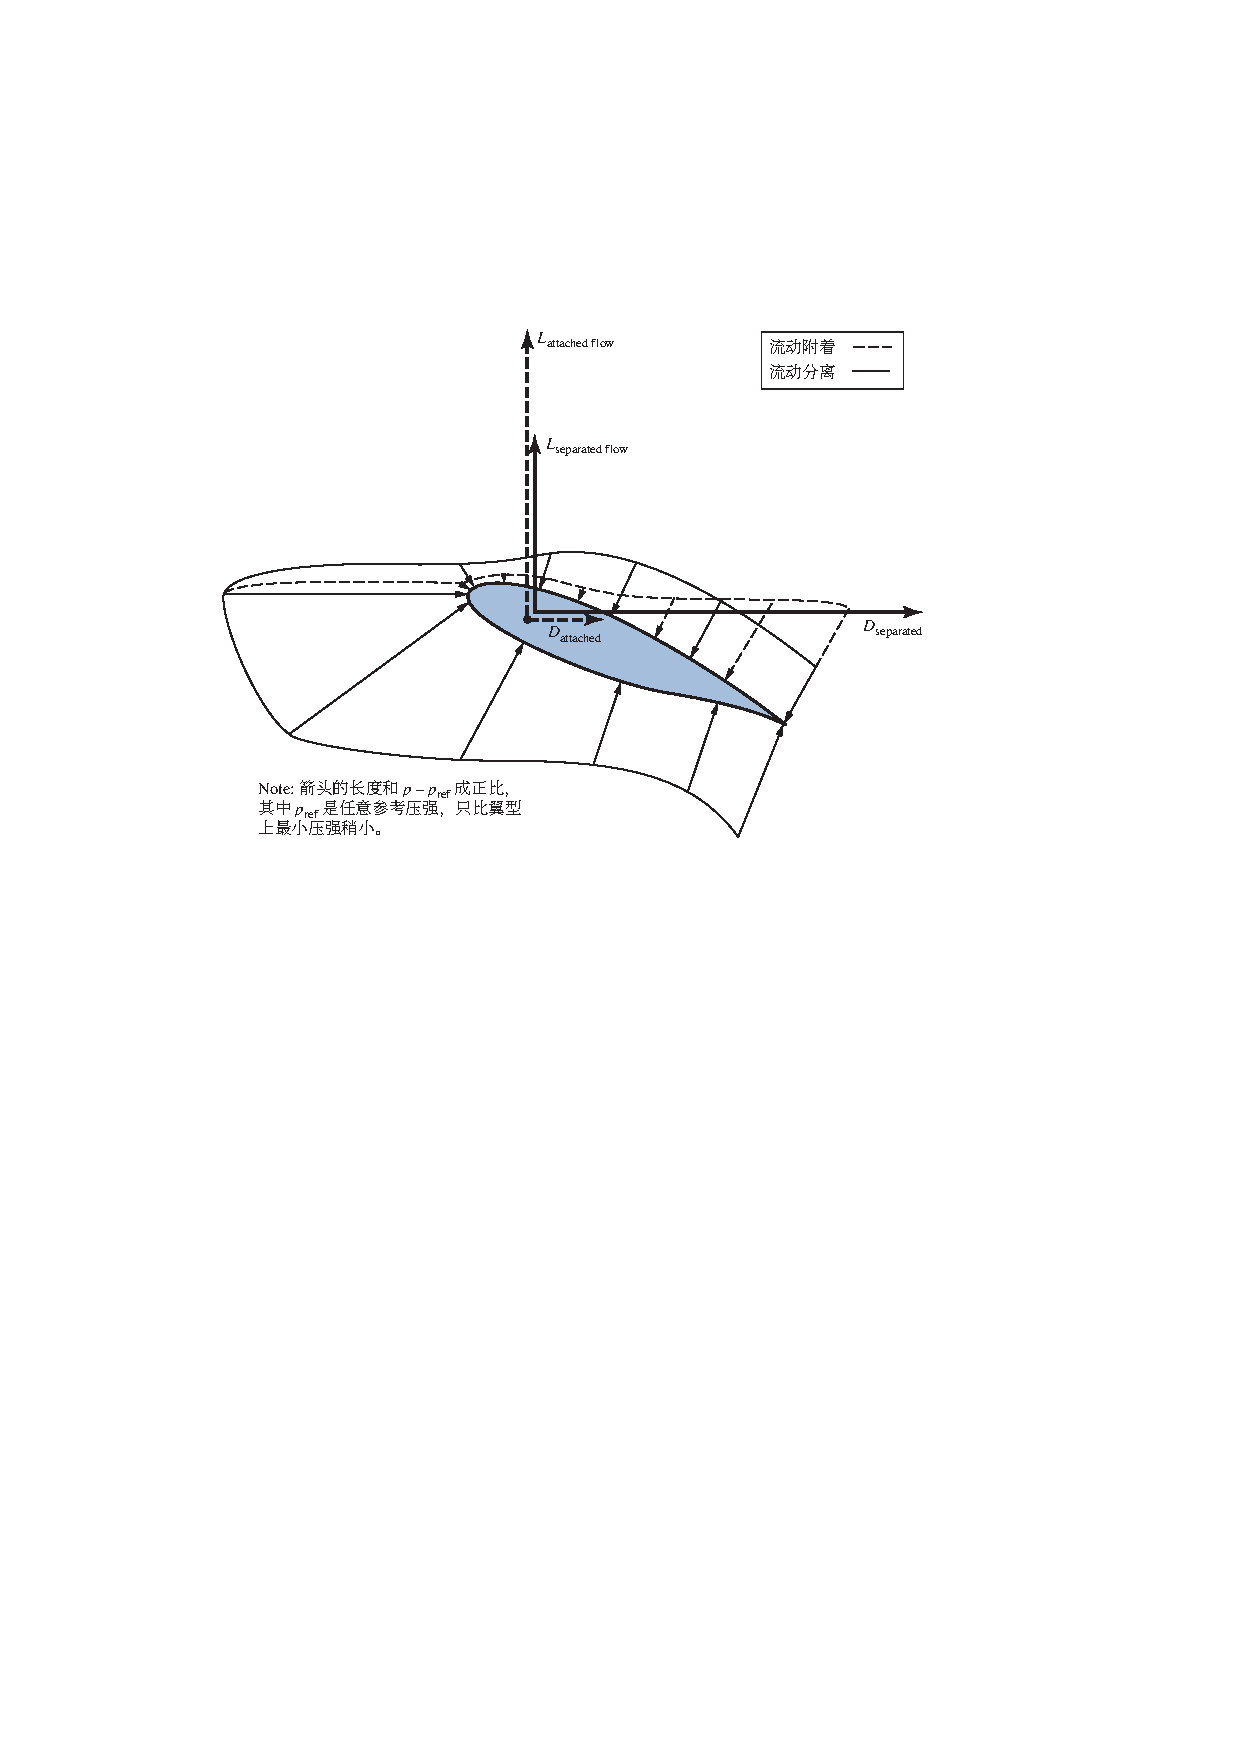
\includegraphics[height=10cm]{./aerodynamics/seprated_flow.pdf}
  \caption{流动分离与流动附着时的对比}
  \label{fig:sepratedflow}
\end{figure}
图中,在非常大攻角下,有着流动分离情况的压强
分布是实线,没有流动分离的情况是虚线。箭头的
长度代表了压强的大小。其中,流动分离的情况下,
压强分布曲线的形状像一个口袋,这使得压强分布
更容易可视化了。如果流动没有分离,压强分布就
是虚线表示的那样。图中的实线箭头和虚线箭头应
该被仔细的对比。它们可以解释流动分离造成的两
个后果。第一个后果是升力的减小。气动升力来源
于压强分布在竖直方向上的净分量(假设自由来流
的方向是水平的)。大升力可以在下表面的压强非
常大而上表面的压强非常小的情况下获得。流动分
离不会影响下表面的压强分布。对比上翼面前缘点
下游的的实线和虚线箭头,可以发现在流动分离的
时候,实现箭头代表了更大的压强。这些压强是向
下作用的,因此升力要减小。

那么为什么气流会从翼型表面分离呢?简而言之,
在逆压梯度区,沿着流线运动的流体微团不得不顶
着增加的压强运动。结果就是,流体微团将会在逆
压梯度的影响下减速。对于边界层外面的流体微团
来说,它们的速度(或者内能)很大,这没什么太
大的问题。它们可以持续地向下游运动。但是对于
边界层内部的流体微团,它们的速度已经被内部的
摩擦阻力减速到很小了。然而,这些流体微团还要
受逆压梯度的影响,因为压强在翼面的法线方向上
是一样的,但是这些流体微团的速度太小了,所以
不能顺利地通过逆压梯度区。最终,这些流体微团
在下游的某个点就会减速到0 ,然后再往回运动。
这些往回流动的流动就从翼型表面分离了。

\section{失速的再介绍}
前面我们分析了失速的原因,即在大迎角下,气流
从翼型表面分离,造成升力系数急剧减小。通过前
面的讨论,我们知道,在达到失速迎角前,增加迎
角可以增加升力系数,但是一旦超过失速迎角,升
力系数就会急剧减小。但是失速发生主要有两种形
式,一种是{\bfseries 前缘点失速(leading-edge stall)},
另一种是{\bfseries 后缘点失速(tralling-edge stall)}。

前缘点失速主要发生在中等翼型中,也就是相对厚度
在10\%到16\%之间的翼型。这种翼型,流动分离是
突然发生在整个上翼面的,开始气流分离主要发生
在前缘点处。相应的,升力曲线在$c_{l,\max}$处
是尖峰状,跨过失速迎角后,升力系数将急剧下降。

与之相应的是后缘点失速,这种失速特性主要发生
在厚度比较大的翼型中,比如NACA 4412 。和前缘
点失速不同,气流是从后缘点开始分离的,并且随
着攻角的增大,分离点逐渐向前缘点移动。升力曲
线在失速迎角处没有中等厚度的翼型那样陡峭,是
比较平缓的,跨过失速迎角后,升力系数下降的没
那么快。

比较两种失速形式,如下:
\begin{enumerate}
  \item 后缘点失速的升力曲线在最大升力系数处
    是逐渐弯曲的,即相对平滑;而前缘点失速则
    是升力曲线急剧下降的。后缘点失速是比较“
    软”的(原文如此)。
  \item 后缘点失速的最大升力系数的值相对没那
    么大。
  \item 翼型厚度主要影响翼型的最大升力系数,
    这种影响主要反映在相对厚度比较大的翼型和
    中等厚度翼型的失速行为之间。
\end{enumerate}

除了前面所述的两种失速行为之外,还有第三种失
速行为,即和非常薄的翼型对应的失速。这种翼型
在小迎角下,气流就会在前缘点附近开始分离形成
一个小的{\bfseries 分离泡(separation buddle)}。
随后,气流又会在下游重新附着在翼型表面上。随
着攻角的增大,这个分离泡会逐渐变大。增大到某
个攻角后,这个分离泡基本上就覆盖了整个上翼面。
这个迎角的大小就对应着最大升力系数。当迎角在
增大,气流就从上翼面完全分离了。这种翼型的升
力曲线,在失速迎角附近和厚度比较大的翼型相似,
都是比较平缓,但是这种很薄的翼型的最大升力系
是三种翼型中最小的。

升力阻力曲线的可取之处是我们可以用来初步地评
定翼型品质的好坏,即:
\begin{enumerate}
  \item {\bfseries 升阻比(lift-to-drag ratio)}
    $\frac{L}{D }$。
    一个效率很高的翼型在产生升力的同时只产生
    很小的阻力。也就是说,升阻比可以衡量一个
    翼型的气动特性。
  \item 最大升力系数$c_{l,\max}$。一个有效的
    翼型会产生更高的升力系数---至少比牛栏门
    的升力系数要高。
\end{enumerate}

这里最大升力系数值得额外的讨论。对于一个飞行
器,最大升力系数决定了它的失速速度。给出失速
速度的计算公式
\[
  V_{stall}=\sqrt{\frac{2W}{q_\infty S C_{L,\max}}} 
\]
因此,我们有很大的动力去获得更大的升力系数,
要么是为了更小的失速速度,要么是在相同速度下
获得更大的荷载。
 \begin{notice}
 假设飞机在海拔10000 m 的高空,该飞机的设计的
 最大速度是1000 Km/h ,设计的失速速度是200 Km/h 。
 那么飞行员在这个高度下,可以操纵飞机飞行的速
 度区间就是200 -- 1000Km/h,低于失速速度,飞机
 就要发生失速,超过最大速度,飞机就要发生解体。
 因此,更低的失速速度意味着飞行员有更大的操纵
 空间,这款飞机就更容易操控,因为飞机安全飞行
 的速度区间更大。
 \end{notice}
更重要的是,操纵性取决于升力系数的大小。另一
方面,在给定雷诺数的情况下,升力系数主要是翼型
形状的函数。一旦翼型的形状确定了,升力系数的大
小也就被确定了。因此,为了使升力系数超过这个值,
我们必须采取一些特别的方法,比如,前缘缝翼和后
缘襟翼。这些装置叫做{\bfseries 增升装置(high-lift devices)}。

{\bfseries 后缘襟翼(tralling-edge flap)}是后缘
的一部分,铰接在后缘处,可以上下翻转。当后缘襟
翼向下翻转的时候,升力就会增加。这是因为,当襟
翼向下翻转的时候相当于增加了翼型的弯度,从而使
得升力变大。在前面的薄翼理论中,我们知道,零升
迎角是弯度的函数,增大弯度,就会让零升迎角变得
更小,相当于升力曲线向左移动了,这样在同迎角下,
升力系数就变大了。更为重要的是,最大升力系数也
变大了,尽管失速迎角稍稍变小了一点。然而,当迎
角保持$0^\circ$ 时,后缘襟翼向下翻转的角度过大,
这时,流线就不对称了,就容易出现失速那样的情况。

当然,增升装置也可以用在前缘,主要有三种形式,即
前缘缝翼(leading-edge slat),leading-edge droop,
前缘襟翼(leading-edge flap)。前缘缝翼只是一个安
装在前缘的很薄的曲面。气流除了从上翼面流过翼型,
在下翼面的气流会通过缝翼和前缘之间的小缝流往上
翼面,这样就能增加上翼面气流的能量。这股气流叫做
二次流动,它能缓解上翼面的逆压梯度区,因此会延缓
气流从上翼面分离。因此,前缘缝翼增大了失速迎角,
同时提高了最大升力系数。前缘缝翼和后缘襟翼的本质
并不相同,前缘襟翼并没有改变零升攻角的大小。它只是
扩大了升力曲线,即增大了失速迎角,附带提高了最大
升力系数。

在现代的高性能大型飞机上,增升装置经常是几种联合
一起使用。

\section{总结}
前面我们介绍了很多关于低速翼型的知识,接下来,请确保
对于下面总结的知识你是熟悉的。
\begin{summary}
  \begin{enumerate}
    \item 平面内一点$(x,y)$ 由从$a$ 点到$b$ 点的面涡
      诱导的速度势由下式给出
      \[
        \Phi(x,y)=- \frac{1}{2\pi}\int _a^b \theta \gamma(s)\mathrm{d}s
      \]
    \item 面涡的环量
      \[
        \Gamma=\int _a^b \gamma(s)\mathrm{d}s 
      \]
    \item 穿过面涡,切向速度是不连续的,
      \[
        \gamma=u_1 -u_2 
      \] 
    \item 库塔条件:如果后缘角是有限的,那么后缘点就是一个
      驻点;如果后缘是圆角过渡的,那么流过上翼面在后缘点的
      速度和流过下翼面在后缘点的速度是相同的,大小和方向都相等,
      同时,在后缘点处,上翼面的压强和下翼面的压强相等。总结如下
      \[
        \gamma(\mathrm{TE})=0 
      \]
    \item 薄翼理论:用中弧线代替翼型。面涡可以放置在弦线上,同时面涡
      的强度可以改变,在叠加自由来流后,中弧线就是流场中的一条流线,
      同时满足库塔条件。面涡的强度可以用下面的公式计算
      \[
        \frac{1}{2\pi}\int _0^c \frac{\gamma(\xi)\mathrm{d}\xi}{x-\xi}
        =V_\infty \left(\alpha-\frac{\mathrm{d}z}{\mathrm{d}x }\right) 
      \]
    \item 薄翼理论的几个结论
      \begin{enumerate}
        \item 对称翼型
          \begin{enumerate}
            \item $c_l=2\pi \alpha$
            \item 升力线斜率 $\frac{\mathrm{d}c_l}{\mathrm{d}\alpha}=2\pi$
            \item 压心和气动中心重合,且都在四分之一弦线处
            \item $c_{m,\frac{c}{4 }}=c_{m,ac}=0$
          \end{enumerate}
        \item 有弯度的翼型
          \begin{enumerate}
            \item $c_l=2\pi\left[\alpha+\frac{1}{\pi}\int_0^\pi
              \frac{\mathrm{d}z}{\mathrm{d}\alpha}(\cos \theta_0-1)\mathrm{d}\theta_0 \frac{\mathrm{d}z}{\mathrm{d}\alpha}(\cos \theta_0-1)\mathrm{d}\theta_0\right] $
            \item 升力线斜率 $\frac{\mathrm{d}c_l}{\mathrm{d}\alpha}=2\pi$
            \item 气动中心在四分之一弦线处
            \item 压心是随着升力系数变化的
          \end{enumerate}
      \end{enumerate}
  \end{enumerate}
\end{summary}

